\documentclass[serif, aspectratio=169]{beamer}
\usepackage[T1]{fontenc} 
\usepackage{fourier}
\usepackage{hyperref}
\usepackage{latexsym,amsmath,xcolor,multicol,booktabs,calligra}
\usepackage{booktabs} % For better table formatting
\usepackage{graphicx,pstricks,listings,stackengine}
\usepackage{listings}
\usepackage{array} 
\usepackage{colortbl}

\author{Dr.Hajialiasgari}
\title{Machine Learning}
\institute{
    Tehran University \\
    Of\\
    Medical Science
}
\date{\small \today}
\usepackage{UoWstyle}

% Define custom colors and styles for listings
\definecolor{deepblue}{rgb}{0,0,0.5}
\definecolor{deepred}{RGB}{153,0,0}
\definecolor{deepgreen}{rgb}{0,0.5,0}
\definecolor{halfgray}{gray}{0.55}

\lstset{
    basicstyle=\ttfamily\small,
    keywordstyle=\bfseries\color{deepblue},
    emphstyle=\ttfamily\color{deepred},
    stringstyle=\color{deepgreen},
    numbers=left,
    numberstyle=\small\color{halfgray},
    rulesepcolor=\color{red!20!green!20!blue!20},
    frame=shadowbox,
}

\begin{document}

\begin{frame}
    \titlepage
    \vspace*{-0.6cm}
    \begin{figure}[htpb]
        \begin{center}
            \includegraphics[keepaspectratio, scale=0.05]{Tumsl-logo.png}
        \end{center}
    \end{figure}
\end{frame}

\begin{frame}    
\tableofcontents[sectionstyle=show, subsectionstyle=show/shaded/hide, subsubsectionstyle=show/shaded/hide]
\end{frame}

\section{SVM}

\begin{frame}{Overview of SVM}
    \begin{itemize}
        \item Support Vector Machine (SVM) is a supervised machine learning algorithm used for classification and regression tasks.
        \item SVM aims to find the optimal hyperplane that separates data points of different classes with the maximum margin.
        \item It can handle both linearly separable and non-linearly separable data using the kernel trick.
    \end{itemize}
\end{frame}

\begin{frame}{Advantages and Disadvantages of SVM}
    \textbf{Advantages:}
    \begin{itemize}
        \item Effective in high-dimensional spaces.
        \item Works well with clear margin separation.
        \item Versatile with different kernel functions.
    \end{itemize}
    \textbf{Disadvantages:}
    \begin{itemize}
        \item Not suitable for very large datasets.
        \item Requires careful selection of the kernel and regularization parameter.
        \item Sensitive to noise and overlapping classes.
    \end{itemize}
\end{frame}

\begin{frame}{Applications of SVM}
    \begin{itemize}
        \item Text and hypertext categorization.
        \item Image classification and object detection.
        \item Bioinformatics, e.g., cancer classification and protein structure prediction.
        \item Handwriting recognition.
        \item Intrusion detection in cybersecurity.
    \end{itemize}
\end{frame}

\begin{frame}{How SVM Works: Linear SVM}
    \begin{itemize}
        \item SVM separates data into two classes by finding the best hyperplane.
        \item \textbf{Linear SVM:} For linearly separable data, SVM finds a straight hyperplane or a flat plane in higher dimensions to separate classes.
        \item The \textbf{support vectors} are the closest data points to the hyperplane. They define the margin and influence the hyperplane's orientation and position.
        \item SVM maximizes the margin between classes for better generalization.
    \end{itemize}
\end{frame}

\begin{frame}{How SVM Works : Linear SVM (Cont.)}
    The maximum-margin hyperplane, also referred to as the hard margin, is selected based on maximizing the distance between the hyperplane and the nearest data point on each side.
    \centering
    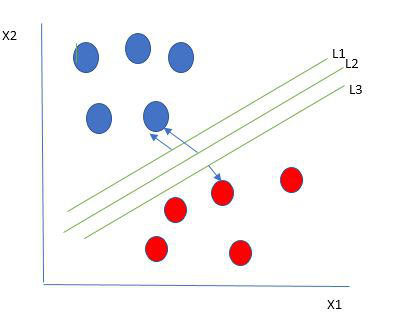
\includegraphics[width=0.45\textwidth]{Capture.jpg}
\end{frame}


\begin{frame}{How SVM Works : Linear SVM (Cont.)}
    What About Now ??
    \centering
    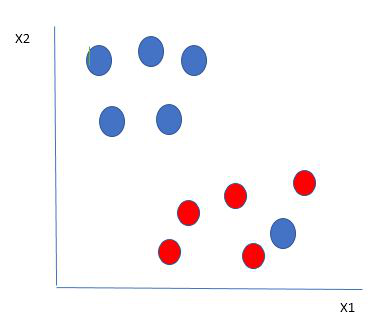
\includegraphics[width=0.45\textwidth]{Capture (1).jpg}
\end{frame}


\begin{frame}{How SVM Works : Linear SVM (Cont.)}
    It’s simple! The blue ball in the boundary of red ones is an outlier of blue balls. The SVM algorithm has the characteristics to ignore the outlier and finds the best hyperplane that maximizes the margin. SVM is robust to outliers.
    \centering
    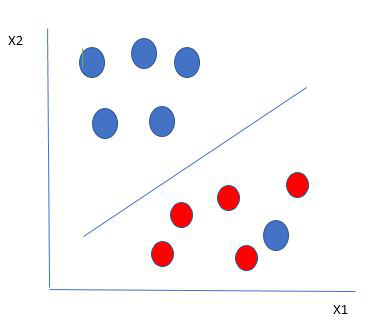
\includegraphics[width=0.45\textwidth]{Capture (2).jpg}
\end{frame}

\begin{frame}{Hyperplane SVM}
    \centering
    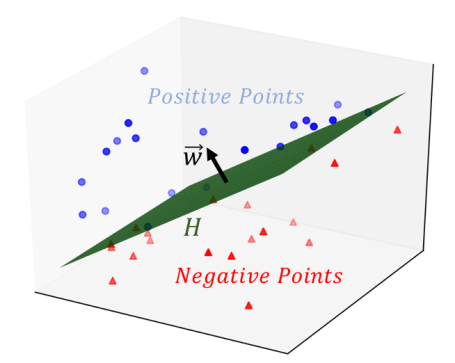
\includegraphics[width=0.45\textwidth]{hyperplanesvm.png}
\end{frame}



\begin{frame}{How SVM Works: Non-Linear SVM}
    \begin{itemize}
        \item \textbf{Non-Linearly Separable Data:} A linear hyperplane cannot separate the classes.
        \item \textbf{Kernel Trick:} SVM maps data to a higher-dimensional space where a linear hyperplane can separate the classes.
        \item Common kernels:
        \begin{itemize}
            \item Linear Kernel: \( K(x, z) = x^T z \)
            \item Polynomial Kernel: \( K(x, z) = (x^T z + c)^d \)
            \item RBF Kernel: \( K(x, z) = \exp(-\gamma ||x - z||^2) \)
        \end{itemize}
    \end{itemize}
\end{frame}

\begin{frame}{How SVM Works : Non-Linear SVM (Cont.)}
    How about this? Can we separate red and blue dot with a linear line ?
    \centering
    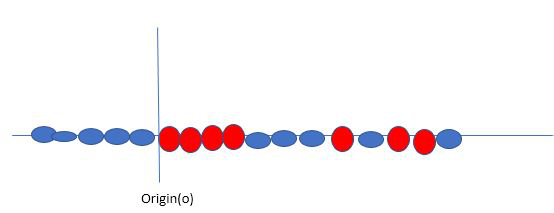
\includegraphics[width=0.45\textwidth]{Capture (3).jpg}
\end{frame}

\begin{frame}{How SVM Works : Non-Linear SVM (Cont.)}
    SVM solves this by creating a new variable using a kernel. We call a point xi on the line and we create a new variable yi as a function of distance from origin o.
    \centering
    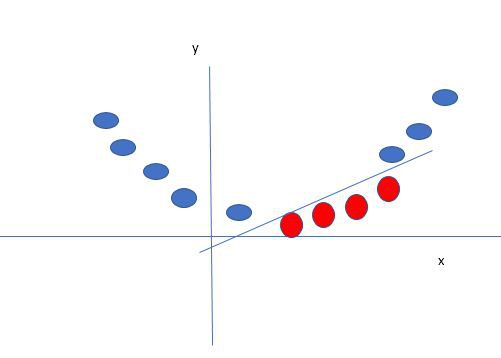
\includegraphics[width=0.45\textwidth]{Capture (4).jpg}
\end{frame}



\begin{frame}{How SVM Works: Margin Maximization}
    \begin{itemize}
        \item The \textbf{margin} is the distance between the hyperplane and the nearest data points from each class.
        \item SVM maximizes this margin while ensuring correct classification.
        \item \textbf{Regularization:} For non-linearly separable data, SVM introduces a parameter \( C \) to balance margin size and classification errors.
    \end{itemize}
\end{frame}

\begin{frame}{How SVM Works: Decision Rule}
    \begin{itemize}
        \item After training, SVM predicts the class label \( y \) for a new sample \( x \) using:
        \[
        y = \text{sign}(w^T x + b)
        \]
        \item \( w \) and \( b \) are learned parameters that define the hyperplane.
        \item The decision rule determines on which side of the hyperplane a data point lies.
    \end{itemize}
\end{frame}

\begin{frame}{Soft VS Hard Margin}
    
    \centering
    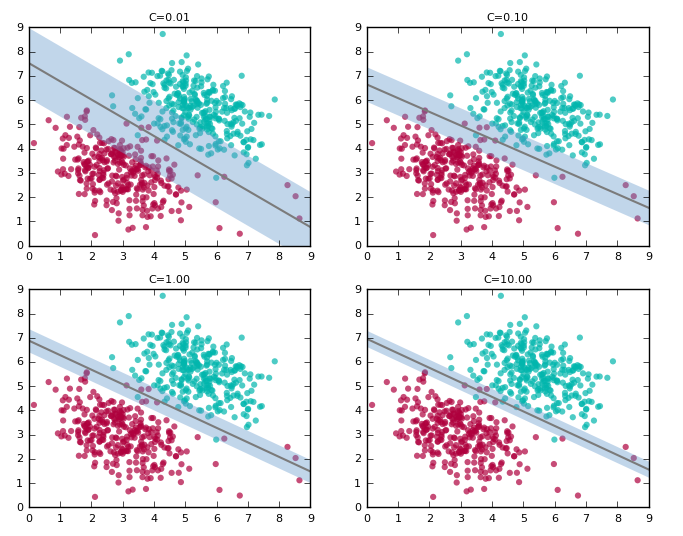
\includegraphics[width=0.5\textwidth]{SVM2.png}
\end{frame}

\section{Naïve Bayes}

% Slide: Conditional Probability
\begin{frame}{Conditional Probability}
    Conditional probability is the probability of an event occurring given that another event has already occurred.
    \begin{equation}
        P(A \mid B) = \frac{P(A \cap B)}{P(B)}
    \end{equation}
\end{frame}

% Slide: Example of Conditional Probability
\begin{frame}{Example: Conditional Probability}
    Suppose 60\% of students in a school like math, and 30\% of students both like math and play chess.
    The probability that a student plays chess given that they like math is:
    \begin{equation}
        P(C \mid M) = \frac{P(C \cap M)}{P(M)} = \frac{0.3}{0.6} = 0.5
    \end{equation}
\end{frame}

% Slide: Bayes' Theorem
\begin{frame}{Bayes' Theorem}
    Bayes' theorem describes how to update probabilities based on new evidence:
    \begin{equation}
        P(A \mid B) = \frac{P(B \mid A) P(A)}{P(B)}
    \end{equation}
\end{frame}

% Slide: Example of Bayes' Theorem
\begin{frame}{Example: Bayes' Theorem}
    Suppose a test for a disease is 95\% accurate when a person has the disease and 90\% accurate when they do not.
    If 1\% of the population has the disease, the probability that a randomly selected person who tested positive actually has the disease is computed as follows:
    \begin{equation}
        P(D \mid T) = \frac{P(T \mid D) P(D)}{P(T)}
    \end{equation}
    \begin{equation}
        = \frac{0.95 \times 0.01}{(0.95 \times 0.01) + (0.1 \times 0.99)} \approx 0.087
    \end{equation}
\end{frame}

\begin{frame}{Naïve Bayes in Classification}
    
    \centering
    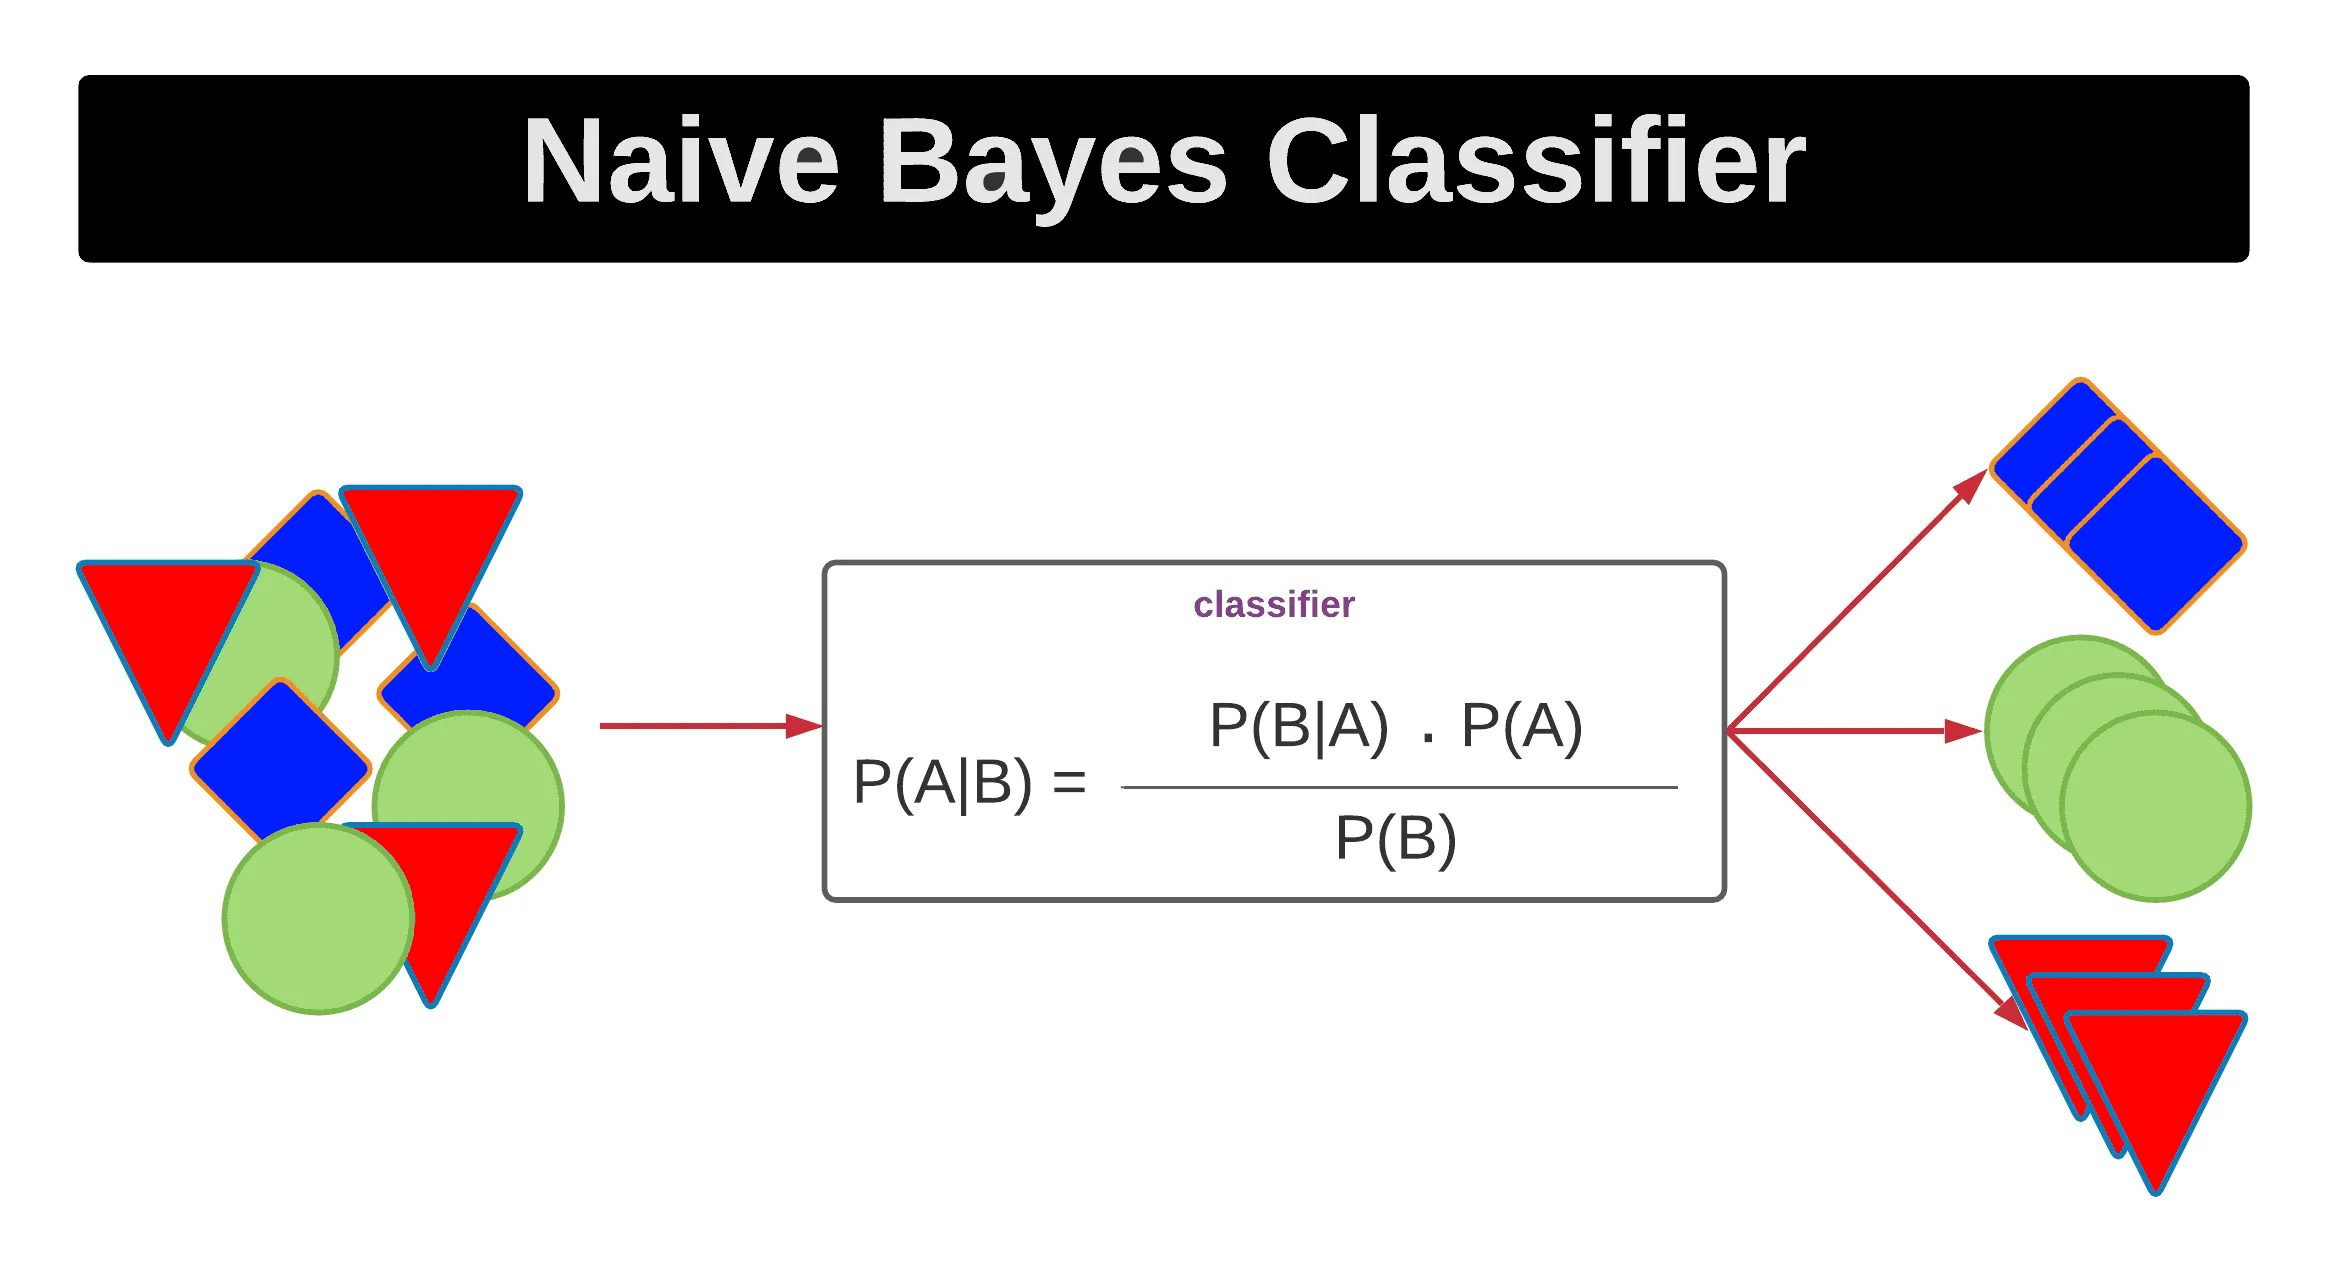
\includegraphics[width=0.9\textwidth]{Navie-Bayes.jpg}
\end{frame}

% Slide: Naïve Bayes in Machine Learning
\begin{frame}{Naïve Bayes in Machine Learning}
    Naïve Bayes is a classification algorithm based on Bayes' theorem with an assumption of independence among features.
    It is commonly used for:
    \begin{itemize}
        \item Spam filtering
        \item Sentiment analysis
        \item Medical diagnosis
    \end{itemize}
\end{frame}

\begin{frame}{How It Works in Medical Diagnosis}
\begin{itemize}
    \item The goal is to predict the presence of a disease given symptoms.
    \item For example, a patient may exhibit symptoms such as fever, cough, and fatigue, and we aim to predict the disease.
\end{itemize}
\end{frame}

\begin{frame}{Bayes' Theorem}
Bayes' Theorem calculates the probability of a disease given symptoms:

\[
P(Disease|Symptom_1, Symptom_2, \dots, Symptom_n) = \frac{P(Disease) \prod_{i=1}^{n} P(Symptom_i|Disease)}{P(Symptom_1, Symptom_2, \dots, Symptom_n)}
\]

\begin{itemize}
    \item \( P(Disease) \): Prior probability of the disease.
    \item \( P(Symptom_i|Disease) \): Likelihood of observing symptom \( Symptom_i \) given the disease.
    \item \( P(Symptom_1, \dots, Symptom_n) \): Evidence, constant across diseases.
\end{itemize}
\end{frame}

\begin{frame}{Conditional Independence Assumption}
Naive Bayes assumes that symptoms (features) are conditionally independent given the disease, simplifying calculations and allowing for efficient handling of many symptoms.
\end{frame}

\begin{frame}{Practical Example}
For a patient with symptoms such as fever, cough, and fatigue, Naive Bayes calculates the probability of different diseases (e.g., flu, pneumonia, COVID-19) based on:
\begin{itemize}
    \item Prior probability of each disease.
    \item Likelihood of each symptom given the disease.
\end{itemize}

\[
P(Disease|Symptoms) = \frac{P(Disease) \prod_{i=1}^{n} P(Symptom_i|Disease)}{P(Symptom_1, \dots, Symptom_n)}
\]
\end{frame}

\begin{frame}{Why It’s Effective}
\begin{itemize}
    \item \textbf{Simplicity}: Despite assuming conditional independence, Naive Bayes often provides accurate results.
    \item \textbf{Efficiency}: It handles large datasets well, typical in medical data.
    \item \textbf{Interpretability}: The model is easy to understand, making it suitable for healthcare applications.
\end{itemize}
\end{frame}

\begin{frame}{Conclusion}
Naive Bayes is an efficient and effective tool for medical diagnosis, predicting diseases based on symptoms, and is widely used in healthcare due to its simplicity and accuracy.
\end{frame}


\begin{frame}
    \begin{center}
        {\Huge\ \color{red}For more information and code check the related notebook}
    \end{center}
\end{frame}


\begin{frame}
    \begin{center}
        {\Huge\ End of Classification}
    \end{center}
\end{frame}

\end{document}

